\begin{task}
\TT{Wyznacz współczynniki trygonometrzycznego szeregu Fouriera dla okresowego sygnału $f(t)$ przedstawionego na rysunku.}{Calculate coefficients of the periodic signal $f(t)$ shown below for the expansion into a trigonometric Fourier series.} 

\begin{figure}[H]
  \centering
  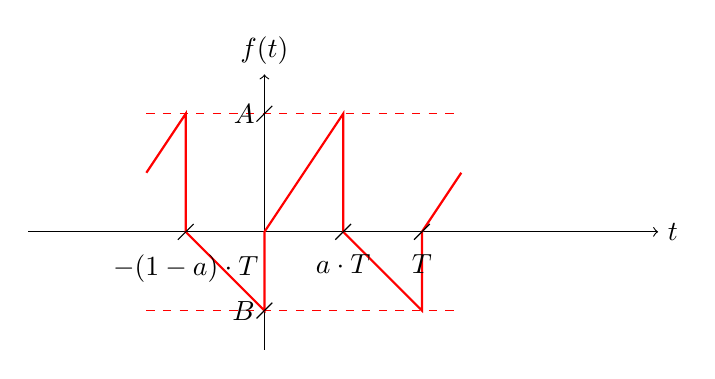
\begin{tikzpicture}
  %\draw (0,0) circle (1in);
  \draw[->] (-3.0,+0.0) -- (+5.0,+0.0) node[right] {$t$};
  \draw[->] (+0.0,-1.5) -- (+0.0,+2.0) node[above] {$f(t)$};
  \draw[-,red, thick] (-1.5,0.75) -- (-1.0,1.5)--(-1.0,0.0) -- (0.0,-1.0) -- (0.0,+0.0) -- (+1.0,+1.5) -- (+1.0,+0.0) -- (+2.0,-1.0) -- (+2.0,+0.0) -- (2.5,0.75);
  \draw[-,red, dashed] (-1.5,1.5) -- (2.5,1.5);
  \draw[-,red, dashed] (-1.5,-1.0) -- (2.5,-1.0);
  %\draw[-] (-1.0-0.1,-0.1)--(-1.0+0.1,0.1) node[midway, below, outer sep=10pt,align=center] {$-\frac{T}{2}$};
  \draw[-] (-1.0-0.1,-0.1)--(-1.0+0.1,0.1) node[midway, below, outer sep=5pt] {$-(1-a)\cdot T$};
  \draw[-] (+1.0-0.1,-0.1)--(+1.0+0.1,0.1) node[midway, below, outer sep=5pt] {$a\cdot T$};
  \draw[-] (+2.0-0.1,-0.1)--(+2.0+0.1,0.1) node[midway, below, outer sep=5pt] {$T$};
  \draw[-] (-0.1,+1.5-0.1)--(+0.1,+1.5+0.1) node[midway, left] {$A$};
  \draw[-] (-0.1,-1.0-0.1)--(+0.1,-1.0+0.1) node[midway, left] {$B$};
  
  \end{tikzpicture}
\end{figure}

\TT{W pierwszej kolejności należy ustalić wzór funkcji przedstawionej na rysunku. Jest to funkcja przedziałowa. W pierwszym okresie możemy ją opisać za pomocą dwóch prostych. Ogólne równanie prostej to:}{First of all, the definition of $f(t)$ signal has to be derived. This is periodic piecewise function, piecewise linear function to be precise. The simplest form of linear function is:}

\begin{equation}
f(t) = m \cdot t + b
\end{equation} 

\TT{W pierwszym okresie, w pierwszej części, wykres funkcji jest prostą przechodzącą przez dwa punkty: $(0,0)$ oraz $(a\cdot T,A)$. Możemy więc napisać układ równań, rozwiązać go i znaleźć nieznane parametry $m$ i $b$: }{In the first interval of the first period (e.g. $t \in (0; a\cdot T)$), linear function crosses two points: $(0,0)$ and $(a\cdot T,A)$. So, in order to derive $m$ and $b$, the following system of the equations has to be solved:} 

\begin{align*}
&\left\{\begin{matrix*}[l]
0 = m\cdot 0 +b\\ 
A = m\cdot a \cdot T +b
\end{matrix*}\right. \\
&\left\{\begin{matrix*}[l]
0 = b\\ 
A = m \cdot a\cdot T +b
\end{matrix*}\right. \\
&\left\{\begin{matrix*}[l]
0 = b\\ 
A = m \cdot a\cdot T +0
\end{matrix*}\right. \\
&\left\{\begin{matrix*}[l]
0 = b\\ 
\frac{A}{a\cdot T} = m
\end{matrix*}\right.
\end{align*}

\TT{Podsumowując, pierwszy odcinek funkcji przedstawionej na rysunku, w pierwszym okresie można opisać wzorem:}{As a result we get:}

\begin{align*}
f(t) = \frac{A}{a \cdot T}\cdot t
\end{align*}

\TT{Drugi odcinek funkcji jest prostą przechodzącą przez następujące dwa punkty: $(a \cdot T,0)$ oraz $(T,-B)$. Możemy więc napisać układ równań, rozwiązać go i znaleźć nieznane parametry $m$ i $b$:}{In the second interval of the first period (e.g. $t \in (a \cdot T;T)$), linear function crosses other two points: $(a \cdot T,0)$ and $(T,-B)$. So, in order to derive $m$ and $b$, the following system of the equations has to be solved:}

\begin{align*}
&\left\{\begin{matrix*}[l]
0 = m\cdot a \cdot T +b\\ 
-B = m\cdot T +b
\end{matrix*}\right. \\
&\left\{\begin{matrix*}[l]
-m \cdot a \cdot T = b\\ 
-B = m \cdot T -m \cdot a \cdot T
\end{matrix*}\right. \\
&\left\{\begin{matrix*}[l]
-m \cdot a \cdot T = b\\ 
-B = m \cdot \left( T - a \cdot T\right)
\end{matrix*}\right. \\
&\left\{\begin{matrix*}[l]
-m \cdot a \cdot T = b\\ 
-\frac{B}{T - a \cdot T} = m
\end{matrix*}\right. \\
&\left\{\begin{matrix*}[l]
\frac{B}{T - a \cdot T} \cdot a \cdot T = b\\ 
-\frac{B}{T - a \cdot T} = m
\end{matrix*}\right. \\
&\left\{\begin{matrix*}[l]
\frac{B}{1 - a} \cdot a = b\\ 
-\frac{B}{T - a \cdot T} = m
\end{matrix*}\right. \\
&\left\{\begin{matrix*}[l]
\frac{B}{1 - a} \cdot a = b\\ 
-\frac{B}{T \cdot \left( 1 - a \right)} = m
\end{matrix*}\right.
\end{align*}

\TT{A więc drugi odcinek funkcji przedstawionej na rysunku w pierwszym okresie, można opisać wzorem:}{As a result, second interval of the first period is described by:}

\begin{align*}
f(t) = -\frac{B}{T \cdot \left(1 - a \right)}\cdot t + \frac{B}{1 - a} \cdot a
\end{align*}

\TT{W związku z tym, całą funkcję w pierwszym okresie można zapisać jako funkcje przedziałową:}{As a result the piecewise linear function in the first period is given by:}

\begin{align*}
f(t) = \left\{\begin{matrix*}[l]
\frac{A}{a \cdot T}\cdot t & dla &t \in (0; a \cdot T)\\ 
-\frac{B}{\left(1 - a \right)\cdot T}\cdot t + \frac{B}{1 - a} \cdot a & dla & t \in (a \cdot T; T)
\end{matrix*}\right.
\end{align*}

\TT{I ogólniej, całą funkcję można wyrazić następującym wzorem:}{For the whole periodic signal $f(t)$ we get:}

\begin{align*}
f(t) = \left\{\begin{matrix*}[l]
\frac{A}{a \cdot T}\cdot \left( t - k\cdot T \right) & dla &t \in (0 + k\cdot T; a \cdot T + k\cdot T)\\ 
-\frac{B}{\left(1 - a\right) \cdot T}\cdot \left( t - k\cdot T \right) + \frac{B}{1 - a} \cdot a & dla & t \in (a \cdot T+ k\cdot T; T+ k\cdot T)
\end{matrix*}\right. \wedge k \in \TT{C}{Z}
\end{align*}

\TT{Współczynnik $a_0$ wyznaczamy ze wzoru}{The $a_0$ coefficient is defined as:}

\begin{equation}
a_0=\frac{1}{T}\int_{T}f(t) \cdot dt
\end{equation}

\TT{Podstawiamy do wzoru wzór naszej funkcji w pierwszym okresie $k=0$}{For the period $t \in \left(0;T\right)$ we get:}

\begin{align*}
a_0&=\frac{1}{T}\int_{T}f(t) \cdot dt=\\
&=\frac{1}{T}\left(\int_{0}^{a\cdot T} \frac{A}{a \cdot T} \cdot t \cdot dt + \int_{a \cdot T}^{T}\left( -\frac{B}{\left(1 -a\right) \cdot T} \cdot t + \frac{B}{1-a}\cdot a\right) \cdot dt\right)=\\
&=\frac{1}{T}\left(\int_{0}^{a\cdot T} \frac{A}{a \cdot T} \cdot t \cdot dt + \int_{a \cdot T}^{T} -\frac{B}{\left(1 -a\right) \cdot T} \cdot t \cdot dt + \int_{a \cdot T}^{T} \frac{B}{1-a}\cdot a \cdot dt\right)=\\
&=\frac{1}{T}\left(\frac{A}{a \cdot T} \cdot \int_{0}^{a\cdot T} t \cdot dt -\frac{B}{\left(1 -a\right) \cdot T} \cdot  \int_{a \cdot T}^{T} t \cdot dt +\frac{B}{1-a}\cdot a \cdot \int_{a \cdot T}^{T} dt\right)=\\
&=\frac{1}{T}\left(\frac{A}{a \cdot T} \cdot \left. \frac{t^2}{2} \right|_{0}^{a\cdot T} -\frac{B}{\left(1 -a\right) \cdot T} \cdot  \left. \frac{t^2}{2} \right|_{a \cdot T}^{T} +\frac{B}{1-a}\cdot a \cdot \left. t\right|_{a \cdot T}^{T}\right)=\\
&=\frac{1}{T}\left(\frac{A}{a \cdot T} \cdot \left( \frac{\left(a\cdot T\right)^2}{2} - \frac{0^2}{2} \right) -\frac{B}{\left(1 -a\right) \cdot T} \cdot  \left( \frac{T^2}{2} -\frac{\left(a\cdot T\right)^2}{2}\right) +\frac{B}{1-a}\cdot a \cdot \left( T - a\cdot T\right)\right)=\\
&=\frac{1}{T}\left(\frac{A}{a \cdot T} \cdot \left( \frac{a^2\cdot T^2}{2} - \frac{0}{2} \right) -\frac{B}{\left(1 -a\right) \cdot T} \cdot  \left( \frac{T^2}{2} -\frac{a^2\cdot T^2}{2}\right) +\frac{B}{1-a}\cdot a \cdot T \cdot \left( 1 - a\right)\right)=\\
&=\frac{1}{T}\left(\frac{A}{a \cdot T} \cdot \left( \frac{a^2\cdot T^2}{2} \right) -\frac{B}{\left(1 -a\right) \cdot T} \cdot T^2 \cdot \left( \frac{1}{2} -\frac{a^2}{2}\right) +B\cdot a \cdot T \right)=\\
&=\frac{1}{T}\left(A \cdot \left( \frac{a\cdot T}{2} \right) -\frac{B}{1 -a} \cdot T \cdot \frac{1}{2}\cdot \left( 1 -a^2\right) +B\cdot a \cdot T \right)=\\
&=\frac{1}{T}\left(A \cdot \frac{a\cdot T}{2} -\frac{B}{1 -a} \cdot T \cdot \frac{1}{2}\cdot \left( 1 -a\right)\cdot \left( 1 +a\right) +B\cdot a \cdot T \right)=\\
&=\frac{1}{T}\left(A \cdot a\cdot T \cdot \frac{1}{2} - B \cdot T \cdot \frac{1}{2}\cdot \left( 1 +a\right) +B\cdot a \cdot T \right)=\\
&=\frac{1}{T}\left(A \cdot a\cdot T \cdot \frac{1}{2} - B \cdot T \cdot \frac{1}{2} - B \cdot T \cdot \frac{1}{2}\cdot a +B\cdot a \cdot T \right)=\\
&=\frac{1}{T}\left(A \cdot a\cdot T \cdot \frac{1}{2} - B \cdot T \cdot \frac{1}{2} + B \cdot T \cdot \frac{1}{2}\cdot a\right)=\\
&=A \cdot a \cdot \frac{1}{2} - B \cdot \frac{1}{2} + B \cdot \frac{1}{2}\cdot a=\\
&=A \cdot a \cdot \frac{1}{2} - B \cdot \frac{1}{2} \left( 1 - a \right)=\\
&=\frac{1}{2} \cdot A \cdot a - \frac{1}{2} \cdot B \cdot \left( 1 - a \right)
\end{align*}

\TT{Wartość współczynnika $a_0$ wynosi}{The $a_0$ coefficient equals} $\frac{1}{2} \cdot A \cdot a - \frac{1}{2} \cdot B \cdot \left( 1 - a \right)$.

\TT{Współczynnik $a_k$ wyznaczamy ze wzoru}{The $a_k$ coefficients are defined as:}

\begin{equation}
 a_k=\frac{2}{T}\int_{T}f(t) \cdot cos\left( k \cdot \frac{2\pi}{T} \cdot t\right) \cdot dt
\end{equation}

\TT{Podstawiamy do wzoru wzór naszej funkcji w pierwszym okresie $k=0$}{For the period $t \in \left(0;T\right)$ we get:}

\begin{align*}
a_k&=\frac{2}{T}\int_{T}f(t) \cdot cos\left( k \cdot \frac{2\pi}{T} \cdot t\right) \cdot dt=\\
&=\frac{2}{T}\cdot\left(\int_{0}^{a\cdot T} \frac{A}{a \cdot T} \cdot t \cdot cos\left( k \cdot \frac{2\pi}{T} \cdot t\right) \cdot dt+\int_{a \cdot T}^{T} \left(-\frac{B}{\left(1-a\right)\cdot T}\cdot t + \frac{B}{1-a}\cdot a\right) \cdot cos\left( k \cdot \frac{2\pi}{T} \cdot t\right) \cdot dt\right)=\\
&=\frac{2}{T}\cdot\left(\int_{0}^{a\cdot T} \frac{A}{a \cdot T} \cdot t \cdot cos\left( k \cdot \frac{2\pi}{T} \cdot t\right) \cdot dt+\int_{a \cdot T}^{T} -\frac{B}{\left(1-a\right)\cdot T}\cdot t \cdot cos\left( k \cdot \frac{2\pi}{T} \cdot t\right) \cdot dt \right. +\\
&+\left. \int_{a \cdot T}^{T} \frac{B}{1-a}\cdot a \cdot cos\left( k \cdot \frac{2\pi}{T} \cdot t\right) \cdot dt\right)=\\
&=\frac{2}{T}\cdot\left( \frac{A}{a \cdot T} \cdot \int_{0}^{a\cdot T} t \cdot cos\left( k \cdot \frac{2\pi}{T} \cdot t\right) \cdot dt -\frac{B}{\left(1-a\right)\cdot T}\cdot \int_{a \cdot T}^{T} t \cdot cos\left( k \cdot \frac{2\pi}{T} \cdot t\right) \cdot dt \right. +\\
&+\left. \frac{B}{1-a}\cdot a \cdot \int_{a \cdot T}^{T} cos\left( k \cdot \frac{2\pi}{T} \cdot t\right) \cdot dt\right)=\\
&=\left\{\begin{array}{l}
z = k \cdot \frac{2\pi}{T} \cdot t \\
dz = k \cdot \frac{2\pi}{T} \cdot dt \\
\frac{dz}{k \cdot \frac{2\pi}{T}} = dt
\end{array}\right\}=\\
&=\frac{2}{T}\cdot\left( \frac{A}{a \cdot T} \cdot \int_{0}^{a\cdot T} t \cdot cos\left( k \cdot \frac{2\pi}{T} \cdot t\right) \cdot dt -\frac{B}{\left(1-a\right)\cdot T}\cdot \int_{a \cdot T}^{T} t \cdot cos\left( k \cdot \frac{2\pi}{T} \cdot t\right) \cdot dt \right. +\\
&+\left. \frac{B}{1-a}\cdot a \cdot \int_{a \cdot T}^{T} cos\left(z\right) \cdot \frac{dz}{k \cdot \frac{2\pi}{T}}\right)=\\
&=\frac{2}{T}\cdot\left( \frac{A}{a \cdot T} \cdot \int_{0}^{a\cdot T} t \cdot cos\left( k \cdot \frac{2\pi}{T} \cdot t\right) \cdot dt -\frac{B}{\left(1-a\right)\cdot T}\cdot \int_{a \cdot T}^{T} t \cdot cos\left( k \cdot \frac{2\pi}{T} \cdot t\right) \cdot dt \right. +\\
&+\left. \frac{B}{1-a}\cdot a \cdot \frac{1}{k \cdot \frac{2\pi}{T}} \int_{a \cdot T}^{T} cos\left(z\right) \cdot dz\right)=\\
&=\frac{2}{T}\cdot\left( \frac{A}{a \cdot T} \cdot \int_{0}^{a\cdot T} t \cdot cos\left( k \cdot \frac{2\pi}{T} \cdot t\right) \cdot dt -\frac{B}{\left(1-a\right)\cdot T}\cdot \int_{a \cdot T}^{T} t \cdot cos\left( k \cdot \frac{2\pi}{T} \cdot t\right) \cdot dt \right. +\\
&+\left. \frac{B}{1-a}\cdot a \cdot \frac{T}{k \cdot 2\pi} \left. sin\left(z\right) \right|_{a \cdot T}^{T}\right)=\\
&=\frac{2}{T}\cdot\left( \frac{A}{a \cdot T} \cdot \int_{0}^{a\cdot T} t \cdot cos\left( k \cdot \frac{2\pi}{T} \cdot t\right) \cdot dt -\frac{B}{\left(1-a\right)\cdot T}\cdot \int_{a \cdot T}^{T} t \cdot cos\left( k \cdot \frac{2\pi}{T} \cdot t\right) \cdot dt \right. +\\
&+\left. \frac{B}{1-a}\cdot a \cdot \frac{T}{k \cdot 2\pi} \left. sin\left(k \cdot \frac{2\pi}{T} \cdot t\right) \right|_{a \cdot T}^{T}\right)=\\
&=\frac{2}{T}\cdot\left( \frac{A}{a \cdot T} \cdot \int_{0}^{a\cdot T} t \cdot cos\left( k \cdot \frac{2\pi}{T} \cdot t\right) \cdot dt -\frac{B}{\left(1-a\right)\cdot T}\cdot \int_{a \cdot T}^{T} t \cdot cos\left( k \cdot \frac{2\pi}{T} \cdot t\right) \cdot dt \right. +\\
&+\left. \frac{B}{1-a}\cdot a \cdot \frac{T}{k \cdot 2\pi} \left( sin\left(k \cdot \frac{2\pi}{T} \cdot T\right) - sin\left(k \cdot \frac{2\pi}{T} \cdot a \cdot T\right) \right)\right)=\\
&=\left\{\begin{array}{ll}
u = t & dv = cos\left( k \cdot \frac{2\pi}{T} \cdot t\right) \cdot dt \\
du = dt & v = \frac{1}{k \cdot \frac{2\pi}{T}} \cdot sin\left( k \cdot \frac{2\pi}{T} \cdot t\right)
\end{array}\right\}=\\
&=\frac{2}{T}\cdot\left( \frac{A}{a \cdot T} \cdot \left( \left. t \cdot \frac{1}{k \cdot \frac{2\pi}{T}} \cdot sin\left( k \cdot \frac{2\pi}{T} \cdot t\right)
\right|_{0}^{a\cdot T} - \int_{0}^{a\cdot T} \frac{1}{k \cdot \frac{2\pi}{T}} \cdot sin\left( k \cdot \frac{2\pi}{T} \cdot t\right) \cdot dt\right) \right. + \\
&-\left.\frac{B}{\left(1-a\right)\cdot T}\cdot \left( \left. t \cdot \frac{1}{k \cdot \frac{2\pi}{T}} \cdot sin\left( k \cdot \frac{2\pi}{T} \cdot t\right) \right|_{a \cdot T}^{T} - \int_{a \cdot T}^{T}  \frac{1}{k \cdot \frac{2\pi}{T}} \cdot sin\left( k \cdot \frac{2\pi}{T} \cdot t\right) \cdot dt \right)\right. +\\
&+\left. \frac{B}{1-a}\cdot a \cdot \frac{T}{k \cdot 2\pi} \left( sin\left(k \cdot \frac{2\pi}{T} \cdot T\right) - sin\left(k \cdot \frac{2\pi}{T} \cdot a \cdot T\right) \right)\right)=\\
&=\frac{2}{T}\cdot\left( \frac{A}{a \cdot T} \cdot \left( \left. t \cdot \frac{1}{k \cdot \frac{2\pi}{T}} \cdot sin\left( k \cdot \frac{2\pi}{T} \cdot t\right)
\right|_{0}^{a\cdot T} - \frac{1}{k \cdot \frac{2\pi}{T}} \cdot \int_{0}^{a\cdot T} sin\left( k \cdot \frac{2\pi}{T} \cdot t\right) \cdot dt\right) \right. + \\
&-\left.\frac{B}{\left(1-a\right)\cdot T}\cdot \left( \left. t \cdot \frac{1}{k \cdot \frac{2\pi}{T}} \cdot sin\left( k \cdot \frac{2\pi}{T} \cdot t\right) \right|_{a \cdot T}^{T} - \frac{1}{k \cdot \frac{2\pi}{T}} \cdot \int_{a \cdot T}^{T}  sin\left( k \cdot \frac{2\pi}{T} \cdot t\right) \cdot dt \right)\right. +\\
&+\left. \frac{B}{1-a}\cdot a \cdot \frac{T}{k \cdot 2\pi} \left( sin\left(k \cdot \frac{2\pi}{T} \cdot T\right) - sin\left(k \cdot \frac{2\pi}{T} \cdot a \cdot T\right) \right)\right)=\\
&=\left\{\begin{array}{l}
z = k \cdot \frac{2\pi}{T} \cdot t \\
dz = k \cdot \frac{2\pi}{T} \cdot dt \\
\frac{dz}{k \cdot \frac{2\pi}{T}} = dt
\end{array}\right\}=\\
&=\frac{2}{T}\cdot\left( \frac{A}{a \cdot T} \cdot \left( \left. t \cdot \frac{1}{k \cdot \frac{2\pi}{T}} \cdot sin\left( k \cdot \frac{2\pi}{T} \cdot t\right)
\right|_{0}^{a\cdot T} - \frac{1}{k \cdot \frac{2\pi}{T}} \cdot \int_{0}^{a\cdot T} sin\left(z\right) \cdot \frac{dz}{k \cdot \frac{2\pi}{T}}\right) \right. + \\
&-\left.\frac{B}{\left(1-a\right)\cdot T}\cdot \left( \left. t \cdot \frac{1}{k \cdot \frac{2\pi}{T}} \cdot sin\left( k \cdot \frac{2\pi}{T} \cdot t\right) \right|_{a \cdot T}^{T} - \frac{1}{k \cdot \frac{2\pi}{T}} \cdot \int_{a \cdot T}^{T}  sin\left( z\right) \cdot \frac{dz}{k \cdot \frac{2\pi}{T}} \right)\right. +\\
&+\left. \frac{B}{1-a}\cdot a \cdot \frac{T}{k \cdot 2\pi} \left( sin\left(k \cdot 2\pi\right) - sin\left(k \cdot 2\pi \cdot a\right) \right)\right)=\\
&=\frac{2}{T}\cdot\left( \frac{A}{a \cdot T} \cdot \left( \left( a\cdot T \cdot \frac{1}{k \cdot \frac{2\pi}{T}} \cdot sin\left( k \cdot \frac{2\pi}{T} \cdot a\cdot T\right)
- 0 \cdot \frac{1}{k \cdot \frac{2\pi}{T}} \cdot sin\left( k \cdot \frac{2\pi}{T} \cdot -\right)\right) \right.\right.+ \\
&- \left. \left. \frac{1}{\left(k \cdot \frac{2\pi}{T}\right)^2} \cdot \int_{0}^{a\cdot T} sin\left(z\right) \cdot dz \right) \right. + \\
&-\left.\frac{B}{\left(1-a\right)\cdot T}\cdot \left( \left( T \cdot \frac{1}{k \cdot \frac{2\pi}{T}} \cdot sin\left( k \cdot \frac{2\pi}{T} \cdot T\right) - a\cdot T \cdot \frac{1}{k \cdot \frac{2\pi}{T}} \cdot sin\left( k \cdot \frac{2\pi}{T} \cdot a\cdot T\right)\right) \right. \right.+ \\
&- \left. \left. \frac{1}{\left(k \cdot \frac{2\pi}{T}\right)^2} \cdot \int_{a \cdot T}^{T}  sin\left( z\right) \cdot dz \right)\right. +\\
&+\left. \frac{B}{1-a}\cdot a \cdot \frac{T}{k \cdot 2\pi} \left( 0 - sin\left(k \cdot 2\pi \cdot a\right) \right)\right)=\\
&=\frac{2}{T}\cdot\left( \frac{A}{a \cdot T} \cdot \left( \left( a\cdot T \cdot \frac{T}{k \cdot 2\pi} \cdot sin\left( k \cdot 2\pi \cdot a\right)
- 0 \right) \right.\right.+ \\
&- \left. \left. \frac{1}{k^2 \cdot \frac{4\pi^2}{T^2}} \cdot \left. \left(-cos\left(z\right) \right) \right|_{0}^{a\cdot T} \right) \right. + \\
&-\left.\frac{B}{\left(1-a\right)\cdot T}\cdot \left( \left( T \cdot \frac{T}{k \cdot 2\pi} \cdot sin\left( k \cdot 2\pi \right) - a\cdot T \cdot \frac{T}{k \cdot 2\pi} \cdot sin\left( k \cdot 2\pi \cdot a \right)\right) \right. \right.+ \\
&- \left. \left. \frac{1}{k^2 \cdot \frac{4\pi^2}{T^2}} \cdot \left. \left(-cos\left( z\right) \right)\right|_{a \cdot T}^{T}  \right)\right. +\\
&+\left. \frac{B}{1-a}\cdot a \cdot \frac{T}{k \cdot 2\pi} \left(- sin\left(k \cdot 2\pi \cdot a\right) \right)\right)=\\
&=\frac{2}{T}\cdot\left( \frac{A}{a \cdot T} \cdot \left( a \cdot \frac{T^2}{k \cdot 2\pi} \cdot sin\left( k \cdot 2\pi \cdot a\right) \right.\right.+ \\
&- \left. \left. \frac{T^2}{k^2 \cdot 4\pi^2} \cdot \left. \left(-cos\left(k \cdot \frac{2\pi}{T} \cdot t\right) \right) \right|_{0}^{a\cdot T} \right) \right. + \\
&-\left.\frac{B}{\left(1-a\right)\cdot T}\cdot \left( \frac{T^2}{k \cdot 2\pi} \cdot 0 - a \cdot \frac{T^2}{k \cdot 2\pi} \cdot sin\left( k \cdot 2\pi \cdot a \right) \right. \right.+ \\
&- \left. \left. \frac{T^2}{k^2 \cdot 4\pi^2} \cdot \left. \left(-cos\left( k \cdot \frac{2\pi}{T} \cdot t\right) \right)\right|_{a \cdot T}^{T}  \right)\right. +\\
&-\left. \frac{B}{1-a}\cdot a \cdot \frac{T}{k \cdot 2\pi} \cdot sin\left(k \cdot 2\pi \cdot a\right) \right)=\\
&=\frac{2}{T}\cdot\left( \frac{A}{a \cdot T} \cdot \left( a \cdot \frac{T^2}{k \cdot 2\pi} \cdot sin\left( k \cdot 2\pi \cdot a\right) \right.\right.+ \\
&- \left. \left. \frac{T^2}{k^2 \cdot 4\pi^2} \cdot \left(-cos\left(k \cdot \frac{2\pi}{T} \cdot a \cdot T\right) + cos\left(k \cdot \frac{2\pi}{T} \cdot 0\right) \right) \right) \right. + \\
&-\left.\frac{B}{\left(1-a\right)\cdot T}\cdot \left( 0 - a \cdot \frac{T^2}{k \cdot 2\pi} \cdot sin\left( k \cdot 2\pi \cdot a \right) \right. \right.+ \\
&- \left. \left. \frac{T^2}{k^2 \cdot 4\pi^2} \cdot \left(-cos\left( k \cdot \frac{2\pi}{T} \cdot T\right) + cos\left( k \cdot \frac{2\pi}{T} \cdot a \cdot T\right) \right)  \right)\right. +\\
&-\left. \frac{B}{1-a}\cdot a \cdot \frac{T}{k \cdot 2\pi} \cdot sin\left(k \cdot 2\pi \cdot a\right) \right)=\\
&=\frac{2}{T}\cdot\left( \frac{A}{a \cdot T} \cdot \left( a \cdot \frac{T^2}{k \cdot 2\pi} \cdot sin\left( k \cdot 2\pi \cdot a\right) - \frac{T^2}{k^2 \cdot 4\pi^2} \cdot \left(-cos\left(k \cdot 2\pi \cdot a \right) + cos\left(0\right) \right) \right) \right. + \\
&-\left.\frac{B}{\left(1-a\right)\cdot T}\cdot \left( - a \cdot \frac{T^2}{k \cdot 2\pi} \cdot sin\left( k \cdot 2\pi \cdot a \right) - \frac{T^2}{k^2 \cdot 4\pi^2} \cdot \left(-cos\left( k \cdot 2\pi\right) + cos\left( k \cdot 2\pi \cdot a \right) \right)  \right)\right. +\\
&-\left. \frac{B}{1-a}\cdot a \cdot \frac{T}{k \cdot 2\pi} \cdot sin\left(k \cdot 2\pi \cdot a\right) \right)=\\
&=\frac{2}{T}\cdot\left( \frac{A}{a \cdot T} \cdot T^2 \left( a \cdot \frac{1}{k \cdot 2\pi} \cdot sin\left( k \cdot 2\pi \cdot a\right) - \frac{1}{k^2 \cdot 4\pi^2} \cdot \left(-cos\left(k \cdot 2\pi \cdot a \right) + 1 \right) \right) \right. + \\
&-\left.\frac{B}{\left(1-a\right)\cdot T}\cdot T^2 \left( - a \cdot \frac{1}{k \cdot 2\pi} \cdot sin\left( k \cdot 2\pi \cdot a \right) - \frac{1}{k^2 \cdot 4\pi^2} \cdot \left(-1 + cos\left( k \cdot 2\pi \cdot a \right) \right)  \right)\right. +\\
&-\left. \frac{B}{1-a}\cdot a \cdot \frac{T}{k \cdot 2\pi} \cdot sin\left(k \cdot 2\pi \cdot a\right) \right)=\\
&=\frac{2}{T}\cdot\left( \frac{A}{a} \cdot T \left( a \cdot \frac{1}{k \cdot 2\pi} \cdot sin\left( k \cdot 2\pi \cdot a\right) - \frac{1}{k^2 \cdot 4\pi^2} \cdot \left(1 -cos\left(k \cdot 2\pi \cdot a \right)\right) \right) \right. + \\
&+\left.\frac{B}{1-a}\cdot T \left(a \cdot \frac{1}{k \cdot 2\pi} \cdot sin\left( k \cdot 2\pi \cdot a \right) - \frac{1}{k^2 \cdot 4\pi^2} \cdot \left(1 - cos\left( k \cdot 2\pi \cdot a \right) \right)  \right)\right. +\\
&-\left. \frac{B}{1-a}\cdot a \cdot \frac{T}{k \cdot 2\pi} \cdot sin\left(k \cdot 2\pi \cdot a\right) \right)=\\
&= \frac{2\cdot A}{a} \left( \frac{a}{k \cdot 2\pi} \cdot sin\left( k \cdot 2\pi \cdot a\right) - \frac{1}{k^2 \cdot 4\pi^2} \cdot \left(1 -cos\left(k \cdot 2\pi \cdot a \right)\right) \right) + \\
&+\frac{2 \cdot B}{1-a} \left(\frac{a}{k \cdot 2\pi} \cdot sin\left( k \cdot 2\pi \cdot a \right) - \frac{1}{k^2 \cdot 4\pi^2} \cdot \left(1 - cos\left( k \cdot 2\pi \cdot a \right) \right)  \right) +\\
&- \frac{2\cdot B}{1-a}\cdot \frac{a}{k \cdot 2\pi} \cdot sin\left(k \cdot 2\pi \cdot a\right)=\\
&= \frac{2\cdot A}{a} \cdot \frac{a}{k \cdot 2\pi} \cdot sin\left( k \cdot 2\pi \cdot a\right) - \frac{2\cdot A}{a}  \cdot \frac{1}{k^2 \cdot 4\pi^2} \cdot \left(1 -cos\left(k \cdot 2\pi \cdot a \right)\right) + \\
&+\frac{2 \cdot B}{1-a} \cdot \frac{a}{k \cdot 2\pi} \cdot sin\left( k \cdot 2\pi \cdot a \right) - \frac{2 \cdot B}{1-a} \cdot \frac{1}{k^2 \cdot 4\pi^2} \cdot \left(1 - cos\left( k \cdot 2\pi \cdot a \right) \right) +\\
&- \frac{2\cdot B}{1-a}\cdot \frac{a}{k \cdot 2\pi} \cdot sin\left(k \cdot 2\pi \cdot a\right)=\\
&= \frac{A}{k \cdot \pi} \cdot sin\left( k \cdot 2\pi \cdot a\right) + \\
& - \frac{A}{a}  \cdot \frac{1}{k^2 \cdot 2\pi^2} \cdot \left(1 -cos\left(k \cdot 2\pi \cdot a \right)\right) + \\
& - \frac{B}{1-a} \cdot \frac{1}{k^2 \cdot 2\pi^2} \cdot \left(1 - cos\left( k \cdot 2\pi \cdot a \right) \right)\\
&= \frac{A}{k \cdot \pi} \cdot sin\left( k \cdot 2\pi \cdot a\right) + \\
& - \frac{A}{a}  \cdot \frac{1}{k^2 \cdot \pi^2} \cdot \frac{1}{2} \cdot \left(1 -cos\left(k \cdot 2\pi \cdot a \right)\right) + \\
& - \frac{B}{1-a} \cdot \frac{1}{k^2 \cdot \pi^2} \cdot \frac{1}{2} \cdot \left(1 - cos\left( k \cdot 2\pi \cdot a \right) \right)\\
&=\left\{\begin{array}{ll}
\frac{1}{2}\cdot \left(1 - cos\left( x\right)\right) = sin^2\left(\frac{x}{2}\right) 
\end{array}\right\}=\\
&= \frac{A}{k \cdot \pi} \cdot sin\left( k \cdot 2\pi \cdot a\right) + \\
& - \frac{A}{a}  \cdot \frac{1}{k^2 \cdot \pi^2} \cdot sin^2\left(k \cdot \pi \cdot a \right) + \\
& - \frac{B}{1-a} \cdot \frac{1}{k^2 \cdot \pi^2} \cdot sin^2\left( k \cdot \pi \cdot a \right)\\
&= \frac{A}{k \cdot \pi} \cdot sin\left( k \cdot 2\pi \cdot a\right) - \left( \frac{A}{a} + \frac{B}{1-a}\right) \cdot \frac{1}{k^2 \cdot \pi^2} \cdot sin^2\left(k \cdot \pi \cdot a \right)
\end{align*}

\TT{Wartość współczynnika $a_k$ wynosi}{The $a_k$ coefficients equal to} $\frac{A}{k \cdot \pi} \cdot sin\left( k \cdot 2\pi \cdot a\right) - \left( \frac{A}{a} + \frac{B}{1-a}\right) \cdot \frac{1}{k^2 \cdot \pi^2} \cdot sin^2\left(k \cdot \pi \cdot a \right)$.

\TT{Współczynnik $b_k$ wyznaczamy ze wzoru}{The $b_k$ coefficients are defined as:}

\begin{equation}
b_k=\frac{2}{T}\int_{T}f(t) \cdot sin\left( k \cdot \frac{2\pi}{T} \cdot t\right) \cdot dt
\end{equation}

\TT{Podstawiamy do wzoru wzór naszej funkcji w pierwszym okresie $k=0$}{For the period $t \in \left(0;T\right)$ we get:}

\begin{align*}
b_k&=\frac{2}{T}\int_{T}f(t) \cdot sin\left( k \cdot \frac{2\pi}{T} \cdot t\right) \cdot dt=\\
&=\frac{2}{T}\cdot\left(\int_{0}^{a\cdot T} \frac{A}{a \cdot T} \cdot t \cdot sin\left( k \cdot \frac{2\pi}{T} \cdot t\right) \cdot dt+\int_{a \cdot T}^{T} \left(-\frac{B}{\left(1-a\right)\cdot T}\cdot t + \frac{B}{1-a}\cdot a\right) \cdot sin\left( k \cdot \frac{2\pi}{T} \cdot t\right) \cdot dt\right)=\\
&=\frac{2}{T}\cdot\left(\int_{0}^{a\cdot T} \frac{A}{a \cdot T} \cdot t \cdot sin\left( k \cdot \frac{2\pi}{T} \cdot t\right) \cdot dt+\int_{a \cdot T}^{T} -\frac{B}{\left(1-a\right)\cdot T}\cdot t \cdot sin\left( k \cdot \frac{2\pi}{T} \cdot t\right) \cdot dt \right. +\\
&+\left. \int_{a \cdot T}^{T} \frac{B}{1-a}\cdot a \cdot sin\left( k \cdot \frac{2\pi}{T} \cdot t\right) \cdot dt\right)=\\
&=\frac{2}{T}\cdot\left( \frac{A}{a \cdot T} \cdot \int_{0}^{a\cdot T} t \cdot sin\left( k \cdot \frac{2\pi}{T} \cdot t\right) \cdot dt -\frac{B}{\left(1-a\right)\cdot T}\cdot \int_{a \cdot T}^{T} t \cdot sin\left( k \cdot \frac{2\pi}{T} \cdot t\right) \cdot dt \right. +\\
&+\left. \frac{B}{1-a}\cdot a \cdot \int_{a \cdot T}^{T} sin\left( k \cdot \frac{2\pi}{T} \cdot t\right) \cdot dt\right)=\\
&=\left\{\begin{array}{l}
z = k \cdot \frac{2\pi}{T} \cdot t \\
dz = k \cdot \frac{2\pi}{T} \cdot dt \\
\frac{dz}{k \cdot \frac{2\pi}{T}} = dt
\end{array}\right\}=\\
&=\frac{2}{T}\cdot\left( \frac{A}{a \cdot T} \cdot \int_{0}^{a\cdot T} t \cdot sin\left( k \cdot \frac{2\pi}{T} \cdot t\right) \cdot dt -\frac{B}{\left(1-a\right)\cdot T}\cdot \int_{a \cdot T}^{T} t \cdot sin\left( k \cdot \frac{2\pi}{T} \cdot t\right) \cdot dt \right. +\\
&+\left. \frac{B}{1-a}\cdot a \cdot \int_{a \cdot T}^{T} sin\left(z\right) \cdot \frac{dz}{k \cdot \frac{2\pi}{T}}\right)=\\
&=\frac{2}{T}\cdot\left( \frac{A}{a \cdot T} \cdot \int_{0}^{a\cdot T} t \cdot sin\left( k \cdot \frac{2\pi}{T} \cdot t\right) \cdot dt -\frac{B}{\left(1-a\right)\cdot T}\cdot \int_{a \cdot T}^{T} t \cdot sin\left( k \cdot \frac{2\pi}{T} \cdot t\right) \cdot dt \right. +\\
&+\left. \frac{B}{1-a}\cdot a \cdot \frac{1}{k \cdot \frac{2\pi}{T}} \int_{a \cdot T}^{T} sin\left(z\right) \cdot dz\right)=\\
&=\frac{2}{T}\cdot\left( \frac{A}{a \cdot T} \cdot \int_{0}^{a\cdot T} t \cdot sin\left( k \cdot \frac{2\pi}{T} \cdot t\right) \cdot dt -\frac{B}{\left(1-a\right)\cdot T}\cdot \int_{a \cdot T}^{T} t \cdot sin\left( k \cdot \frac{2\pi}{T} \cdot t\right) \cdot dt \right. +\\
&-\left. \frac{B}{1-a}\cdot a \cdot \frac{T}{k \cdot 2\pi} \left. cos\left(z\right) \right|_{a \cdot T}^{T}\right)=\\
&=\frac{2}{T}\cdot\left( \frac{A}{a \cdot T} \cdot \int_{0}^{a\cdot T} t \cdot sin\left( k \cdot \frac{2\pi}{T} \cdot t\right) \cdot dt -\frac{B}{\left(1-a\right)\cdot T}\cdot \int_{a \cdot T}^{T} t \cdot sin\left( k \cdot \frac{2\pi}{T} \cdot t\right) \cdot dt \right. +\\
&-\left. \frac{B}{1-a}\cdot a \cdot \frac{T}{k \cdot 2\pi} \left. cos\left(k \cdot \frac{2\pi}{T} \cdot t\right) \right|_{a \cdot T}^{T}\right)=\\
&=\frac{2}{T}\cdot\left( \frac{A}{a \cdot T} \cdot \int_{0}^{a\cdot T} t \cdot sin\left( k \cdot \frac{2\pi}{T} \cdot t\right) \cdot dt -\frac{B}{\left(1-a\right)\cdot T}\cdot \int_{a \cdot T}^{T} t \cdot sin\left( k \cdot \frac{2\pi}{T} \cdot t\right) \cdot dt \right. +\\
&-\left. \frac{B}{1-a}\cdot a \cdot \frac{T}{k \cdot 2\pi} \left( cos\left(k \cdot \frac{2\pi}{T} \cdot T\right) - cos\left(k \cdot \frac{2\pi}{T} \cdot a \cdot T\right) \right)\right)=\\
&=\left\{\begin{array}{ll}
u = t & dv = sin\left( k \cdot \frac{2\pi}{T} \cdot t\right) \cdot dt \\
du = dt & v = -\frac{1}{k \cdot \frac{2\pi}{T}} \cdot cos\left( k \cdot \frac{2\pi}{T} \cdot t\right)
\end{array}\right\}=\\
&=\frac{2}{T}\cdot\left( \frac{A}{a \cdot T} \cdot \left( \left. - t \cdot \frac{1}{k \cdot \frac{2\pi}{T}} \cdot cos\left( k \cdot \frac{2\pi}{T} \cdot t\right)
\right|_{0}^{a\cdot T} + \int_{0}^{a\cdot T} \frac{1}{k \cdot \frac{2\pi}{T}} \cdot cos\left( k \cdot \frac{2\pi}{T} \cdot t\right) \cdot dt\right) \right. + \\
&-\left.\frac{B}{\left(1-a\right)\cdot T}\cdot \left( \left. -t \cdot \frac{1}{k \cdot \frac{2\pi}{T}} \cdot cos\left( k \cdot \frac{2\pi}{T} \cdot t\right) \right|_{a \cdot T}^{T} + \int_{a \cdot T}^{T}  \frac{1}{k \cdot \frac{2\pi}{T}} \cdot cos\left( k \cdot \frac{2\pi}{T} \cdot t\right) \cdot dt \right)\right. +\\
&-\left. \frac{B}{1-a}\cdot a \cdot \frac{T}{k \cdot 2\pi} \left( cos\left(k \cdot \frac{2\pi}{T} \cdot T\right) - cos\left(k \cdot \frac{2\pi}{T} \cdot a \cdot T\right) \right)\right)=\\
&=\frac{2}{T}\cdot\left( \frac{A}{a \cdot T} \cdot \left( \left. - t \cdot \frac{1}{k \cdot \frac{2\pi}{T}} \cdot cos\left( k \cdot \frac{2\pi}{T} \cdot t\right)
\right|_{0}^{a\cdot T} + \frac{1}{k \cdot \frac{2\pi}{T}} \cdot \int_{0}^{a\cdot T} cos\left( k \cdot \frac{2\pi}{T} \cdot t\right) \cdot dt\right) \right. + \\
&-\left.\frac{B}{\left(1-a\right)\cdot T}\cdot \left( \left.- t \cdot \frac{1}{k \cdot \frac{2\pi}{T}} \cdot cos\left( k \cdot \frac{2\pi}{T} \cdot t\right) \right|_{a \cdot T}^{T} + \frac{1}{k \cdot \frac{2\pi}{T}} \cdot \int_{a \cdot T}^{T} cos\left( k \cdot \frac{2\pi}{T} \cdot t\right) \cdot dt \right)\right. +\\
&-\left. \frac{B}{1-a}\cdot a \cdot \frac{T}{k \cdot 2\pi} \left( cos\left(k \cdot \frac{2\pi}{T} \cdot T\right) - cos\left(k \cdot \frac{2\pi}{T} \cdot a \cdot T\right) \right)\right)=\\
&=\left\{\begin{array}{l}
z = k \cdot \frac{2\pi}{T} \cdot t \\
dz = k \cdot \frac{2\pi}{T} \cdot dt \\
\frac{dz}{k \cdot \frac{2\pi}{T}} = dt
\end{array}\right\}=\\
&=\frac{2}{T}\cdot\left( \frac{A}{a \cdot T} \cdot \left( \left. -t \cdot \frac{1}{k \cdot \frac{2\pi}{T}} \cdot cos\left( k \cdot \frac{2\pi}{T} \cdot t\right)
\right|_{0}^{a\cdot T} + \frac{1}{k \cdot \frac{2\pi}{T}} \cdot \int_{0}^{a\cdot T} cos\left(z\right) \cdot \frac{dz}{k \cdot \frac{2\pi}{T}}\right) \right. + \\
&-\left.\frac{B}{\left(1-a\right)\cdot T}\cdot \left( \left. -t \cdot \frac{1}{k \cdot \frac{2\pi}{T}} \cdot cos\left( k \cdot \frac{2\pi}{T} \cdot t\right) \right|_{a \cdot T}^{T} + \frac{1}{k \cdot \frac{2\pi}{T}} \cdot \int_{a \cdot T}^{T}  cos\left( z\right) \cdot \frac{dz}{k \cdot \frac{2\pi}{T}} \right)\right. +\\
&-\left. \frac{B}{1-a}\cdot a \cdot \frac{T}{k \cdot 2\pi} \left( cos\left(k \cdot 2\pi\right) - cos\left(k \cdot 2\pi \cdot a\right) \right)\right)=\\
&=\frac{2}{T}\cdot\left( \frac{A}{a \cdot T} \cdot \left( \left( - a\cdot T \cdot \frac{1}{k \cdot \frac{2\pi}{T}} \cdot cos\left( k \cdot \frac{2\pi}{T} \cdot a\cdot T\right)
+ 0 \cdot \frac{1}{k \cdot \frac{2\pi}{T}} \cdot cos\left( k \cdot \frac{2\pi}{T} \cdot 0\right)\right) \right.\right.+ \\
&+ \left. \left. \frac{1}{\left(k \cdot \frac{2\pi}{T}\right)^2} \cdot \int_{0}^{a\cdot T} cos\left(z\right) \cdot dz \right) \right. + \\
&-\left.\frac{B}{\left(1-a\right)\cdot T}\cdot \left( \left( - T \cdot \frac{1}{k \cdot \frac{2\pi}{T}} \cdot cos\left( k \cdot \frac{2\pi}{T} \cdot T\right) + a\cdot T \cdot \frac{1}{k \cdot \frac{2\pi}{T}} \cdot cos\left( k \cdot \frac{2\pi}{T} \cdot a\cdot T\right)\right) \right. \right.+ \\
&+ \left. \left. \frac{1}{\left(k \cdot \frac{2\pi}{T}\right)^2} \cdot \int_{a \cdot T}^{T}  cos\left( z\right) \cdot dz \right)\right. +\\
&-\left. \frac{B}{1-a}\cdot a \cdot \frac{T}{k \cdot 2\pi} \cdot \left( 1 - cos\left(k \cdot 2\pi \cdot a\right) \right)\right)=\\
&=\frac{2}{T}\cdot\left( \frac{A}{a \cdot T} \cdot \left( \left( - a\cdot T \cdot \frac{T}{k \cdot 2\pi} \cdot cos\left( k \cdot 2\pi \cdot a\right)
+ 0 \right) \right.\right.+ \\
&+ \left. \left. \frac{1}{k^2 \cdot \frac{4\pi^2}{T^2}} \cdot \left. \left(sin\left(z\right) \right) \right|_{0}^{a\cdot T} \right) \right. + \\
&-\left.\frac{B}{\left(1-a\right)\cdot T}\cdot \left( \left( -T \cdot \frac{T}{k \cdot 2\pi} \cdot cos\left( k \cdot 2\pi \right) + a\cdot T \cdot \frac{T}{k \cdot 2\pi} \cdot cos\left( k \cdot 2\pi \cdot a \right)\right) \right. \right.+ \\
&+ \left. \left. \frac{1}{k^2 \cdot \frac{4\pi^2}{T^2}} \cdot \left. \left(sin\left( z\right) \right)\right|_{a \cdot T}^{T}  \right)\right. +\\
&-\left. \frac{B}{1-a}\cdot a \cdot \frac{T}{k \cdot 2\pi} \cdot \left(1 - cos\left(k \cdot 2\pi \cdot a\right) \right)\right)=\\
&=\frac{2}{T}\cdot\left( \frac{A}{a \cdot T} \cdot \left( - a\cdot T \cdot \frac{T}{k \cdot 2\pi} \cdot cos\left( k \cdot 2\pi \cdot a\right) \right.\right.+ \\
&+ \left. \left. \frac{1}{k^2 \cdot \frac{4\pi^2}{T^2}} \cdot \left. \left(sin\left(k \cdot \frac{2\pi}{T} \cdot t\right) \right) \right|_{0}^{a\cdot T} \right) \right. + \\
&-\left.\frac{B}{\left(1-a\right)\cdot T}\cdot \left( \left( -T \cdot \frac{T}{k \cdot 2\pi} \cdot 1 + a\cdot T \cdot \frac{T}{k \cdot 2\pi} \cdot cos\left( k \cdot 2\pi \cdot a \right)\right) \right. \right.+ \\
&+ \left. \left. \frac{1}{k^2 \cdot \frac{4\pi^2}{T^2}} \cdot \left. \left(sin\left( k \cdot \frac{2\pi}{T} \cdot t\right) \right)\right|_{a \cdot T}^{T}  \right)\right. +\\
&-\left. \frac{B}{1-a}\cdot a \cdot \frac{T}{k \cdot 2\pi} \cdot \left(1 - cos\left(k \cdot 2\pi \cdot a\right) \right)\right)=\\
&=\frac{2}{T}\cdot\left( \frac{A}{a \cdot T} \cdot \left( - a\cdot T \cdot \frac{T}{k \cdot 2\pi} \cdot cos\left( k \cdot 2\pi \cdot a\right) \right.\right.+ \\
&+ \left. \left. \frac{1}{k^2 \cdot \frac{4\pi^2}{T^2}} \cdot \left(sin\left(k \cdot \frac{2\pi}{T} \cdot a\cdot T\right) - sin\left(k \cdot \frac{2\pi}{T} \cdot 0\right)\right) \right) \right. + \\
&-\left.\frac{B}{\left(1-a\right)\cdot T}\cdot \left(T \cdot \frac{T}{k \cdot 2\pi} \cdot \left( -1 + a \cdot cos\left( k \cdot 2\pi \cdot a \right)\right) \right. \right.+ \\
&+ \left. \left. \frac{1}{k^2 \cdot \frac{4\pi^2}{T^2}} \cdot \left(sin\left( k \cdot \frac{2\pi}{T} \cdot T\right) - sin\left( k \cdot \frac{2\pi}{T} \cdot a \cdot T\right)\right) \right)\right. +\\
&-\left. \frac{B}{1-a}\cdot a \cdot \frac{T}{k \cdot 2\pi} \cdot \left(1 - cos\left(k \cdot 2\pi \cdot a\right) \right)\right)=\\
&=\frac{2}{T}\cdot\left( \frac{A}{a \cdot T} \cdot \left( - a\cdot \frac{T^2}{k \cdot 2\pi} \cdot cos\left( k \cdot 2\pi \cdot a\right) \right.\right.+ \\
&+ \left. \left. \frac{T^2}{k^2 \cdot 4\pi^2} \cdot \left(sin\left(k \cdot 2\pi \cdot a\right) - sin\left(0\right)\right) \right) \right. + \\
&-\left.\frac{B}{\left(1-a\right)\cdot T}\cdot \left( \frac{T^2}{k \cdot 2\pi} \cdot \left( -1 + a \cdot cos\left( k \cdot 2\pi \cdot a \right)\right) \right. \right.+ \\
&+ \left. \left. \frac{T^2}{k^2 \cdot 4\pi^2} \cdot \left(sin\left( k \cdot 2\pi\right) - sin\left( k \cdot 2\pi \cdot a\right)\right) \right)\right. +\\
&-\left. \frac{B}{1-a}\cdot a \cdot \frac{T}{k \cdot 2\pi} \cdot \left(1 - cos\left(k \cdot 2\pi \cdot a\right) \right)\right)=\\
&=\frac{2}{T}\cdot\left( \frac{A}{a \cdot T} \cdot \left( - a\cdot \frac{T^2}{k \cdot 2\pi} \cdot cos\left( k \cdot 2\pi \cdot a\right) \right.\right.+ \\
&+ \left. \left. \frac{T^2}{k^2 \cdot 4\pi^2} \cdot \left(sin\left(k \cdot 2\pi \cdot a\right) - 0\right) \right) \right. + \\
&-\left.\frac{B}{\left(1-a\right)\cdot T}\cdot \left( \frac{T^2}{k \cdot 2\pi} \cdot \left( -1 + a \cdot cos\left( k \cdot 2\pi \cdot a \right)\right) \right. \right.+ \\
&+ \left. \left. \frac{T^2}{k^2 \cdot 4\pi^2} \cdot \left(0 - sin\left( k \cdot 2\pi \cdot a\right)\right) \right)\right. +\\
&-\left. \frac{B}{1-a}\cdot a \cdot \frac{T}{k \cdot 2\pi} \cdot \left(1 - cos\left(k \cdot 2\pi \cdot a\right) \right)\right)=\\
&=\frac{2}{T}\cdot\left( \frac{A}{a \cdot T} \cdot \left( - a\cdot \frac{T^2}{k \cdot 2\pi} \cdot cos\left( k \cdot 2\pi \cdot a\right) + \frac{T^2}{k^2 \cdot 4\pi^2} \cdot sin\left(k \cdot 2\pi \cdot a\right) \right) \right. + \\
&-\left.\frac{B}{\left(1-a\right)\cdot T}\cdot \left( \frac{T^2}{k \cdot 2\pi} \cdot \left( -1 + a \cdot cos\left( k \cdot 2\pi \cdot a \right)\right) - \frac{T^2}{k^2 \cdot 4\pi^2} \cdot sin\left( k \cdot 2\pi \cdot a\right)\right) \right. +\\
&-\left. \frac{B}{1-a}\cdot a \cdot \frac{T}{k \cdot 2\pi} \cdot \left(1 - cos\left(k \cdot 2\pi \cdot a\right) \right)\right)=\\
&=\frac{2}{T}\cdot\left( \frac{A}{a \cdot T} \cdot \frac{T^2}{2} \cdot \left( - a\cdot \frac{1}{k \cdot \pi} \cdot cos\left( k \cdot 2\pi \cdot a\right) + \frac{1}{k^2 \cdot 2\pi^2} \cdot sin\left(k \cdot 2\pi \cdot a\right) \right) \right. + \\
&-\left.\frac{B}{\left(1-a\right)\cdot T}\cdot \frac{T^2}{2}\cdot\left( \frac{1}{k \cdot \pi} \cdot \left( -1 + a \cdot cos\left( k \cdot 2\pi \cdot a \right)\right) - \frac{1}{k^2 \cdot 2\pi^2} \cdot sin\left( k \cdot 2\pi \cdot a\right)\right) \right. +\\
&-\left. \frac{B}{1-a}\cdot a \cdot \frac{T}{k \cdot 2\pi} \cdot \left(1 - cos\left(k \cdot 2\pi \cdot a\right) \right)\right)=\\
&=\frac{2}{T}\cdot \frac{A}{a \cdot T} \cdot \frac{T^2}{2} \cdot \left( - a\cdot \frac{1}{k \cdot \pi} \cdot cos\left( k \cdot 2\pi \cdot a\right) + \frac{1}{k^2 \cdot 2\pi^2} \cdot sin\left(k \cdot 2\pi \cdot a\right) \right) + \\
&-\frac{2}{T}\cdot \frac{B}{\left(1-a\right)\cdot T}\cdot \frac{T^2}{2}\cdot\left( \frac{1}{k \cdot \pi} \cdot \left( -1 + a \cdot cos\left( k \cdot 2\pi \cdot a \right)\right) - \frac{1}{k^2 \cdot 2\pi^2} \cdot sin\left( k \cdot 2\pi \cdot a\right)\right) +\\
&- \frac{2}{T}\cdot \frac{B}{1-a}\cdot a \cdot \frac{T}{k \cdot 2\pi} \cdot \left(1 - cos\left(k \cdot 2\pi \cdot a\right) \right)=\\
&=\frac{A}{a}\cdot \left( - a\cdot \frac{1}{k \cdot \pi} \cdot cos\left( k \cdot 2\pi \cdot a\right) + \frac{1}{k^2 \cdot 2\pi^2} \cdot sin\left(k \cdot 2\pi \cdot a\right) \right) + \\
&-\frac{B}{1-a}\cdot \left( \frac{1}{k \cdot \pi} \cdot \left( -1 + a \cdot cos\left( k \cdot 2\pi \cdot a \right)\right) - \frac{1}{k^2 \cdot 2\pi^2} \cdot sin\left( k \cdot 2\pi \cdot a\right)\right) +\\
&- \frac{B}{1-a}\cdot a \cdot \frac{1}{k \cdot \pi} \cdot \left(1 - cos\left(k \cdot 2\pi \cdot a\right) \right)=\\
&= - \frac{A}{a}\cdot a\cdot \frac{1}{k \cdot \pi} \cdot cos\left( k \cdot 2\pi \cdot a\right) + \frac{A}{a}\cdot \frac{1}{k^2 \cdot 2\pi^2} \cdot sin\left(k \cdot 2\pi \cdot a\right) + \\
& -\frac{B}{1-a}\cdot \frac{1}{k \cdot \pi} \cdot \left( -1 + a \cdot cos\left( k \cdot 2\pi \cdot a \right)\right) + \frac{B}{1-a}\cdot \frac{1}{k^2 \cdot 2\pi^2} \cdot sin\left( k \cdot 2\pi \cdot a\right) +\\
&- \frac{B}{1-a}\cdot a \cdot \frac{1}{k \cdot \pi} \cdot \left(1 - cos\left(k \cdot 2\pi \cdot a\right) \right)=\\
&= - \frac{A}{k \cdot \pi} \cdot cos\left( k \cdot 2\pi \cdot a\right) + \frac{A}{a}\cdot \frac{1}{k^2 \cdot 2\pi^2} \cdot sin\left(k \cdot 2\pi \cdot a\right) + \\
& +\frac{B}{1-a}\cdot \frac{1}{k \cdot \pi} -\frac{B}{1-a}\cdot \frac{1}{k \cdot \pi} \cdot a \cdot cos\left( k \cdot 2\pi \cdot a \right) + \frac{B}{1-a}\cdot \frac{1}{k^2 \cdot 2\pi^2} \cdot sin\left( k \cdot 2\pi \cdot a\right) +\\
&- \frac{B}{1-a}\cdot a \cdot \frac{1}{k \cdot \pi} + \frac{B}{1-a}\cdot a \cdot \frac{1}{k \cdot \pi} \cdot cos\left(k \cdot 2\pi \cdot a\right)=\\
&= - \frac{A}{k \cdot \pi} \cdot cos\left( k \cdot 2\pi \cdot a\right) + \frac{A}{a}\cdot \frac{1}{k^2 \cdot 2\pi^2} \cdot sin\left(k \cdot 2\pi \cdot a\right) + \\
& + \frac{B}{1-a}\cdot \frac{1}{k^2 \cdot 2\pi^2} \cdot sin\left( k \cdot 2\pi \cdot a\right) +\\
& +\frac{B}{1-a}\cdot \frac{1}{k \cdot \pi} - \frac{B}{1-a}\cdot a \cdot \frac{1}{k \cdot \pi} =\\
&= - \frac{A}{k \cdot \pi} \cdot cos\left( k \cdot 2\pi \cdot a\right) + \left(\frac{A}{a}+ \frac{B}{1-a}\right)\cdot \frac{1}{k^2 \cdot 2\pi^2} \cdot sin\left(k \cdot 2\pi \cdot a\right) + \\
& +\frac{B}{1-a}\cdot \frac{1}{k \cdot \pi} \cdot \left(1 - a\right) =\\
&= - \frac{A}{k \cdot \pi} \cdot cos\left( k \cdot 2\pi \cdot a\right) + \left(\frac{A}{a}+ \frac{B}{1-a}\right)\cdot \frac{1}{k^2 \cdot 2\pi^2} \cdot sin\left(k \cdot 2\pi \cdot a\right) +\frac{B}{k \cdot \pi}\\
\end{align*}

\TT{Wartość współczynnika $b_k$ wynosi}{The $b_k$ coefficients equal to} $\frac{B}{k \cdot \pi} - \frac{A}{k \cdot \pi} \cdot cos\left( k \cdot 2\pi \cdot a\right) + \left(\frac{A}{a}+ \frac{B}{1-a}\right)\cdot \frac{1}{k^2 \cdot 2\pi^2} \cdot sin\left(k \cdot 2\pi \cdot a\right)$.

\TT{Ostatecznie współczynniki trygonometrycznego szeregu Fouriera dla funkcji przedstawionej na rysunku przyjmują wartości.}{To sum up, coefficients for the expansion into trigonometric Fourier series are given by:}

\begin{align*}
a_0&=\frac{1}{2} \cdot A \cdot a - \frac{1}{2} \cdot B \cdot \left( 1 - a \right)\\
a_k&=\frac{A}{k \cdot \pi} \cdot sin\left( k \cdot 2\pi \cdot a\right) - \left( \frac{A}{a} + \frac{B}{1-a}\right) \cdot \frac{1}{k^2 \cdot \pi^2} \cdot sin^2\left(k \cdot \pi \cdot a \right)\\
b_k&=\frac{B}{k \cdot \pi} - \frac{A}{k \cdot \pi} \cdot cos\left( k \cdot 2\pi \cdot a\right) + \left(\frac{A}{a}+ \frac{B}{1-a}\right)\cdot \frac{1}{k^2 \cdot 2\pi^2} \cdot sin\left(k \cdot 2\pi \cdot a\right)\\
\end{align*}

\TT{Możemy wyznaczyć kilka wartości współczynników $a_k$ i $b_k$:}{The first six coefficients are equal to:}

\begin{table}[H]
  \centering  
  \begin{tabular}{|c|c|c|}
    \hline 
    $k$ & $a_k$ & $b_k$\\ 
    \hline 
    $1$ & $\frac{A}{\pi} \cdot sin\left(2\pi \cdot a\right) - \left( \frac{A}{a} + \frac{B}{1-a}\right) \cdot \frac{1}{\pi^2} \cdot sin^2\left(\pi \cdot a \right)$ & $\frac{B}{\pi} - \frac{A}{\pi} \cdot cos\left(2\pi \cdot a\right) + \left(\frac{A}{a}+ \frac{B}{1-a}\right)\cdot \frac{1}{2\pi^2} \cdot sin\left(2\pi \cdot a\right)$\\
    \hline 
    $2$ & $\frac{A}{2\pi} \cdot sin\left( 4\pi \cdot a\right) - \left( \frac{A}{a} + \frac{B}{1-a}\right) \cdot \frac{1}{4 \pi^2} \cdot sin^2\left(2 \pi \cdot a \right)$ & $\frac{B}{2\pi} - \frac{A}{2\pi} \cdot cos\left( 4\pi \cdot a\right) + \left(\frac{A}{a}+ \frac{B}{1-a}\right)\cdot \frac{1}{8\pi^2} \cdot sin\left(4\pi \cdot a\right)$\\
    \hline 
    $3$ & $\frac{A}{3\pi} \cdot sin\left( 6\pi \cdot a\right) - \left( \frac{A}{a} + \frac{B}{1-a}\right) \cdot \frac{1}{9\pi^2} \cdot sin^2\left(3\pi \cdot a \right)$ & $\frac{B}{3\pi} - \frac{A}{3\pi} \cdot cos\left(6\pi \cdot a\right) + \left(\frac{A}{a}+ \frac{B}{1-a}\right)\cdot \frac{1}{18\pi^2} \cdot sin\left(6\pi \cdot a\right)$\\
    \hline 
    $4$ & $\frac{A}{4\pi} \cdot sin\left( 8\pi \cdot a\right) - \left( \frac{A}{a} + \frac{B}{1-a}\right) \cdot \frac{1}{16\pi^2} \cdot sin^2\left(4\pi \cdot a \right)$ & $\frac{B}{4\pi} - \frac{A}{4\pi} \cdot cos\left(8\pi \cdot a\right) + \left(\frac{A}{a}+ \frac{B}{1-a}\right)\cdot \frac{1}{32\pi^2} \cdot sin\left(8\pi \cdot a\right)$\\
    \hline 
    $5$ & $\frac{A}{5\pi} \cdot sin\left( 10\pi \cdot a\right) - \left( \frac{A}{a} + \frac{B}{1-a}\right) \cdot \frac{1}{25\pi^2} \cdot sin^2\left(5\pi \cdot a \right)$ & $\frac{B}{5\pi} - \frac{A}{5\pi} \cdot cos\left(10\pi \cdot a\right) + \left(\frac{A}{a}+ \frac{B}{1-a}\right)\cdot \frac{1}{50\pi^2} \cdot sin\left(10\pi \cdot a\right)$\\
    \hline 
    $6$ & $\frac{A}{6\pi} \cdot sin\left( 12\pi \cdot a\right) - \left( \frac{A}{a} + \frac{B}{1-a}\right) \cdot \frac{1}{36\pi^2} \cdot sin^2\left(6\pi \cdot a \right)$ & $\frac{B}{6\pi} - \frac{A}{6\pi} \cdot cos\left( 12\pi \cdot a\right) + \left(\frac{A}{a}+ \frac{B}{1-a}\right)\cdot \frac{1}{72\pi^2} \cdot sin\left(12\pi \cdot a\right)$\\ 
    \hline 
  \end{tabular} 
\end{table}

\TT{Podstawiając do wzoru aproksymacyjnego funkcje $f(t)$ możemy wyrazić jako}{Hence, the signal $f(t)$ may be expressed as the sum of the harmonic series}

\begin{equation}
\begin{aligned}
f(t) &= a_0 + \sum_{k=1}^{\infty} \left[ a_k \cdot cos\left( k \cdot \frac{2\pi}{T} \cdot t\right) + b_k \cdot sin\left(k \cdot \frac{2\pi}{T} \cdot t\right)\right]
\end{aligned}
\end{equation}

\TT{W przypadku sumowania do $k_{max}=1$ otrzymujemy:}{A partial approximation of the $f(t)$ signal for $k_{max}=1$ results in:}

\begin{figure}[H]
  \centering
  \begin{tikzpicture}
  
  \tikzmath{
    function a0(\A,\B,\a) {
      return 1/2*\A*\a-1/2*\B*(1-\a);
    };
    function ak(\k,\A,\B,\a) {
    return \A / (\k * 3.141592) * sin(\k*2*180*\a) - (\A/\a+\B/(1-\a))*1/((\k)^2*(3.141592)^2)*(sin(\k*180*\a))^2;
    };
    function bk(\k,\A,\B,\a) {
      return \B/(\k*3.141592)-\A/(\k*3.141592)*cos(\k*2*180*\a)+(\A/\a+\B/(1-\a))*1/((\k)^2*2*(3.141592)^2)*sin(\k*2*180*\a);
    };
  }
  
  %\draw (0,0) circle (1in);
  \draw[->] (-3.0,+0.0) -- (+5.0,+0.0) node[right] {$t$};
  \draw[->] (+0.0,-1.5) -- (+0.0,+1.5) node[above] {$f(t)$};
  %\draw[-,red, thick] (-2.5,+0.0) -- (+0.0,+0.0);
  %\draw[-] (-1.0-0.1,-0.1)--(-1.0+0.1,0.1) node[midway, below, outer sep=10pt,align=center] {$-\frac{T}{2}$};
  \draw[-] (-1.0-0.1,-0.1)--(-1.0+0.1,0.1) node[midway, below, outer sep=5pt,align=center] {$-\frac{T}{2}$};
  \draw[-] (+1.0-0.1,-0.1)--(+1.0+0.1,0.1) node[midway, below, outer sep=5pt] {$a\cdot T$};
  \draw[-] (+2.0-0.1,-0.1)--(+2.0+0.1,0.1) node[midway, below, outer sep=5pt] {$T$};
  \draw[-] (-0.1,1.0-0.1)--(+0.1,1.0+0.1) node[midway, left] {$A$};
  
  \draw[scale=1.0,domain=-4:4.0,samples=100,smooth,variable=\x,red,thick] plot ({\x},{a0(1,1,0.5)+ak(1,1,1,0.5)*cos(\x*180.0/3.141592*1.0*3.141592/1.0)+bk(1,1,1,0.5)*sin(\x*180.0/3.141592*1.0*3.141592/1.0)});
  \end{tikzpicture}
\end{figure}

\TT{W przypadku sumowania do $k_{max}=2$ otrzymujemy:}{A partial approximation of the $f(t)$ signal for $k_{max}=2$ results in:}

\begin{figure}[H]
  \centering
  \begin{tikzpicture}
  
  \tikzmath{
    function a0(\A,\B,\a) {
      return 1/2*\A*\a-1/2*\B*(1-\a);
    };
    function ak(\k,\A,\B,\a) {
      return \A / (\k * 3.141592) * sin(\k*2*180*\a) - (\A/\a+\B/(1-\a))*1/((\k)^2*(3.141592)^2)*(sin(\k*180*\a))^2;
    };
    function bk(\k,\A,\B,\a) {
      return \B/(\k*3.141592)-\A/(\k*3.141592)*cos(\k*2*180*\a)+(\A/\a+\B/(1-\a))*1/((\k)^2*2*(3.141592)^2)*sin(\k*2*180*\a);
    };
  }
  
  %\draw (0,0) circle (1in);
  \draw[->] (-3.0,+0.0) -- (+5.0,+0.0) node[right] {$t$};
  \draw[->] (+0.0,-1.5) -- (+0.0,+1.5) node[above] {$f(t)$};
  %\draw[-,red, thick] (-2.5,+0.0) -- (+0.0,+0.0);
  %\draw[-] (-1.0-0.1,-0.1)--(-1.0+0.1,0.1) node[midway, below, outer sep=10pt,align=center] {$-\frac{T}{2}$};
  \draw[-] (-1.0-0.1,-0.1)--(-1.0+0.1,0.1) node[midway, below, outer sep=5pt,align=center] {$-\frac{T}{2}$};
  \draw[-] (+1.0-0.1,-0.1)--(+1.0+0.1,0.1) node[midway, below, outer sep=5pt] {$a\cdot T$};
  \draw[-] (+2.0-0.1,-0.1)--(+2.0+0.1,0.1) node[midway, below, outer sep=5pt] {$T$};
  \draw[-] (-0.1,1.0-0.1)--(+0.1,1.0+0.1) node[midway, left] {$A$};
  
  \draw[scale=1.0,domain=-4:4.0,samples=100,smooth,variable=\x,red,thick] plot ({\x},{a0(1,1,0.5)+ak(1,1,1,0.5)*cos(\x*180.0/3.141592*1.0*3.141592/1.0)+bk(1,1,1,0.5)*sin(\x*180.0/3.141592*1.0*3.141592/1.0)+ak(2,1,1,0.5)*cos(\x*180.0/3.141592*2.0*3.141592/1.0)+bk(2,1,1,0.5)*sin(\x*180.0/3.141592*2.0*3.141592/1.0)});
  \end{tikzpicture}
\end{figure}

\TT{W przypadku sumowania do $k_{max}=4$ otrzymujemy:}{A partial approximation of the $f(t)$ signal for $k_{max}=4$ results in:}

\begin{figure}[H]
  \centering
  \begin{tikzpicture}
  
  \tikzmath{
    function a0(\A,\B,\a) {
      return 1/2*\A*\a-1/2*\B*(1-\a);
    };
    function ak(\k,\A,\B,\a) {
      return \A / (\k * 3.141592) * sin(\k*2*180*\a) - (\A/\a+\B/(1-\a))*1/((\k)^2*(3.141592)^2)*(sin(\k*180*\a))^2;
    };
    function bk(\k,\A,\B,\a) {
      return \B/(\k*3.141592)-\A/(\k*3.141592)*cos(\k*2*180*\a)+(\A/\a+\B/(1-\a))*1/((\k)^2*2*(3.141592)^2)*sin(\k*2*180*\a);
    };
  }
  
  %\draw (0,0) circle (1in);
  \draw[->] (-3.0,+0.0) -- (+5.0,+0.0) node[right] {$t$};
  \draw[->] (+0.0,-1.5) -- (+0.0,+1.5) node[above] {$f(t)$};
  %\draw[-,red, thick] (-2.5,+0.0) -- (+0.0,+0.0);
  %\draw[-] (-1.0-0.1,-0.1)--(-1.0+0.1,0.1) node[midway, below, outer sep=10pt,align=center] {$-\frac{T}{2}$};
  \draw[-] (-1.0-0.1,-0.1)--(-1.0+0.1,0.1) node[midway, below, outer sep=5pt,align=center] {$-\frac{T}{2}$};
  \draw[-] (+1.0-0.1,-0.1)--(+1.0+0.1,0.1) node[midway, below, outer sep=5pt] {$a\cdot T$};
  \draw[-] (+2.0-0.1,-0.1)--(+2.0+0.1,0.1) node[midway, below, outer sep=5pt] {$T$};
  \draw[-] (-0.1,1.0-0.1)--(+0.1,1.0+0.1) node[midway, left] {$A$};
  
  \draw[scale=1.0,domain=-4:4.0,samples=100,smooth,variable=\x,red,thick] plot ({\x},{a0(1,1,0.5)+ak(1,1,1,0.5)*cos(\x*180.0/3.141592*1.0*3.141592/1.0)+bk(1,1,1,0.5)*sin(\x*180.0/3.141592*1.0*3.141592/1.0)+ak(2,1,1,0.5)*cos(\x*180.0/3.141592*2.0*3.141592/1.0)+bk(2,1,1,0.5)*sin(\x*180.0/3.141592*2.0*3.141592/1.0)+ak(3,1,1,0.5)*cos(\x*180.0/3.141592*3.0*3.141592/1.0)+bk(3,1,1,0.5)*sin(\x*180.0/3.141592*3.0*3.141592/1.0)+ak(4,1,1,0.5)*cos(\x*180.0/3.141592*4.0*3.141592/1.0)+bk(4,1,1,0.5)*sin(\x*180.0/3.141592*4.0*3.141592/1.0)});
  \end{tikzpicture}
\end{figure}

\TT{W przypadku sumowania do $k_{max}=6$ otrzymujemy:}{A partial approximation of the $f(t)$ signal for $k_{max}=6$ results in:}

\begin{figure}[H]
  \centering
  \begin{tikzpicture}
  
  \tikzmath{
    function a0(\A,\B,\a) {
      return 1/2*\A*\a-1/2*\B*(1-\a);
    };
    function ak(\k,\A,\B,\a) {
      return \A / (\k * 3.141592) * sin(\k*2*180*\a) - (\A/\a+\B/(1-\a))*1/((\k)^2*(3.141592)^2)*(sin(\k*180*\a))^2;
    };
    function bk(\k,\A,\B,\a) {
      return \B/(\k*3.141592)-\A/(\k*3.141592)*cos(\k*2*180*\a)+(\A/\a+\B/(1-\a))*1/((\k)^2*2*(3.141592)^2)*sin(\k*2*180*\a);
    };
  }
  
  %\draw (0,0) circle (1in);
  \draw[->] (-3.0,+0.0) -- (+5.0,+0.0) node[right] {$t$};
  \draw[->] (+0.0,-1.5) -- (+0.0,+1.5) node[above] {$f(t)$};
  %\draw[-,red, thick] (-2.5,+0.0) -- (+0.0,+0.0);
  %\draw[-] (-1.0-0.1,-0.1)--(-1.0+0.1,0.1) node[midway, below, outer sep=10pt,align=center] {$-\frac{T}{2}$};
  \draw[-] (-1.0-0.1,-0.1)--(-1.0+0.1,0.1) node[midway, below, outer sep=5pt,align=center] {$-\frac{T}{2}$};
  \draw[-] (+1.0-0.1,-0.1)--(+1.0+0.1,0.1) node[midway, below, outer sep=5pt] {$a\cdot T$};
  \draw[-] (+2.0-0.1,-0.1)--(+2.0+0.1,0.1) node[midway, below, outer sep=5pt] {$T$};
  \draw[-] (-0.1,1.0-0.1)--(+0.1,1.0+0.1) node[midway, left] {$A$};
  
  \draw[scale=1.0,domain=-4:4.0,samples=300,smooth,variable=\x,red,thick] plot ({\x},{a0(1,1,0.5)+ak(1,1,1,0.5)*cos(\x*180.0/3.141592*1.0*3.141592/1.0)+bk(1,1,1,0.5)*sin(\x*180.0/3.141592*1.0*3.141592/1.0)+ak(2,1,1,0.5)*cos(\x*180.0/3.141592*2.0*3.141592/1.0)+bk(2,1,1,0.5)*sin(\x*180.0/3.141592*2.0*3.141592/1.0)+ak(3,1,1,0.5)*cos(\x*180.0/3.141592*3.0*3.141592/1.0)+bk(3,1,1,0.5)*sin(\x*180.0/3.141592*3.0*3.141592/1.0)+ak(4,1,1,0.5)*cos(\x*180.0/3.141592*4.0*3.141592/1.0)+bk(4,1,1,0.5)*sin(\x*180.0/3.141592*4.0*3.141592/1.0)+ak(5,1,1,0.5)*cos(\x*180.0/3.141592*5.0*3.141592/1.0)+bk(5,1,1,0.5)*sin(\x*180.0/3.141592*5.0*3.141592/1.0)+ak(6,1,1,0.5)*cos(\x*180.0/3.141592*6.0*3.141592/1.0)+bk(6,1,1,0.5)*sin(\x*180.0/3.141592*6.0*3.141592/1.0)});
  \end{tikzpicture}
\end{figure}

\TT{W przypadku sumowania do $k_{max}=12$ otrzymujemy:}{A partial approximation of the $f(t)$ signal for $k_{max}=12$ results in:}

\begin{figure}[H]
  \centering
  \begin{tikzpicture}
  
  \tikzmath{
    function a0(\A,\B,\a) {
      return 1/2*\A*\a-1/2*\B*(1-\a);
    };
    function ak(\k,\A,\B,\a) {
      return \A / (\k * 3.141592) * sin(\k*2*180*\a) - (\A/\a+\B/(1-\a))*1/((\k)^2*(3.141592)^2)*(sin(\k*180*\a))^2;
    };
    function bk(\k,\A,\B,\a) {
      return \B/(\k*3.141592)-\A/(\k*3.141592)*cos(\k*2*180*\a)+(\A/\a+\B/(1-\a))*1/((\k)^2*2*(3.141592)^2)*sin(\k*2*180*\a);
    };
  }
  
  %\draw (0,0) circle (1in);
  \draw[->] (-3.0,+0.0) -- (+5.0,+0.0) node[right] {$t$};
  \draw[->] (+0.0,-1.5) -- (+0.0,+1.5) node[above] {$f(t)$};
  %\draw[-,red, thick] (-2.5,+0.0) -- (+0.0,+0.0);
  %\draw[-] (-1.0-0.1,-0.1)--(-1.0+0.1,0.1) node[midway, below, outer sep=10pt,align=center] {$-\frac{T}{2}$};
  \draw[-] (-1.0-0.1,-0.1)--(-1.0+0.1,0.1) node[midway, below, outer sep=5pt,align=center] {$-\frac{T}{2}$};
  \draw[-] (+1.0-0.1,-0.1)--(+1.0+0.1,0.1) node[midway, below, outer sep=5pt] {$a\cdot T$};
  \draw[-] (+2.0-0.1,-0.1)--(+2.0+0.1,0.1) node[midway, below, outer sep=5pt] {$T$};
  \draw[-] (-0.1,1.0-0.1)--(+0.1,1.0+0.1) node[midway, left] {$A$};
  
  \draw[scale=1.0,domain=-4:4.0,samples=300,smooth,variable=\x,red,thick] plot ({\x},{a0(1,1,0.5)+ak(1,1,1,0.5)*cos(\x*180.0/3.141592*1.0*3.141592/1.0)+bk(1,1,1,0.5)*sin(\x*180.0/3.141592*1.0*3.141592/1.0)+ak(2,1,1,0.5)*cos(\x*180.0/3.141592*2.0*3.141592/1.0)+bk(2,1,1,0.5)*sin(\x*180.0/3.141592*2.0*3.141592/1.0)+ak(3,1,1,0.5)*cos(\x*180.0/3.141592*3.0*3.141592/1.0)+bk(3,1,1,0.5)*sin(\x*180.0/3.141592*3.0*3.141592/1.0)+ak(4,1,1,0.5)*cos(\x*180.0/3.141592*4.0*3.141592/1.0)+bk(4,1,1,0.5)*sin(\x*180.0/3.141592*4.0*3.141592/1.0)+ak(5,1,1,0.5)*cos(\x*180.0/3.141592*5.0*3.141592/1.0)+bk(5,1,1,0.5)*sin(\x*180.0/3.141592*5.0*3.141592/1.0)+ak(6,1,1,0.5)*cos(\x*180.0/3.141592*6.0*3.141592/1.0)+bk(6,1,1,0.5)*sin(\x*180.0/3.141592*6.0*3.141592/1.0)+ak(7,1,1,0.5)*cos(\x*180.0/3.141592*7.0*3.141592/1.0)+bk(7,1,1,0.5)*sin(\x*180.0/3.141592*7.0*3.141592/1.0)+ak(8,1,1,0.5)*cos(\x*180.0/3.141592*8.0*3.141592/1.0)+bk(8,1,1,0.5)*sin(\x*180.0/3.141592*8.0*3.141592/1.0)+ak(9,1,1,0.5)*cos(\x*180.0/3.141592*9.0*3.141592/1.0)+bk(9,1,1,0.5)*sin(\x*180.0/3.141592*9.0*3.141592/1.0)+ak(10,1,1,0.5)*cos(\x*180.0/3.141592*10.0*3.141592/1.0)+bk(10,1,1,0.5)*sin(\x*180.0/3.141592*10.0*3.141592/1.0)+ak(11,1,1,0.5)*cos(\x*180.0/3.141592*11.0*3.141592/1.0)+bk(11,1,1,0.5)*sin(\x*180.0/3.141592*11.0*3.141592/1.0)+ak(12,1,1,0.5)*cos(\x*180.0/3.141592*12.0*3.141592/1.0)+bk(12,1,1,0.5)*sin(\x*180.0/3.141592*12.0*3.141592/1.0)});
  \end{tikzpicture}
\end{figure}

\TT{W przypadku sumowania do $k_{max}=16$ otrzymujemy:}{A partial approximation of the $f(t)$ signal for $k_{max}=16$ results in:}

\begin{figure}[H]
  \centering
  \begin{tikzpicture}
  
  \tikzmath{
    function a0(\A,\B,\a) {
      return 1/2*\A*\a-1/2*\B*(1-\a);
    };
    function ak(\k,\A,\B,\a) {
      return \A / (\k * 3.141592) * sin(\k*2*180*\a) - (\A/\a+\B/(1-\a))*1/((\k)^2*(3.141592)^2)*(sin(\k*180*\a))^2;
    };
    function bk(\k,\A,\B,\a) {
      return \B/(\k*3.141592)-\A/(\k*3.141592)*cos(\k*2*180*\a)+(\A/\a+\B/(1-\a))*1/((\k)^2*2*(3.141592)^2)*sin(\k*2*180*\a);
    };
  }
  
  %\draw (0,0) circle (1in);
  \draw[->] (-3.0,+0.0) -- (+5.0,+0.0) node[right] {$t$};
  \draw[->] (+0.0,-1.5) -- (+0.0,+1.5) node[above] {$f(t)$};
  %\draw[-,red, thick] (-2.5,+0.0) -- (+0.0,+0.0);
  %\draw[-] (-1.0-0.1,-0.1)--(-1.0+0.1,0.1) node[midway, below, outer sep=10pt,align=center] {$-\frac{T}{2}$};
  \draw[-] (-1.0-0.1,-0.1)--(-1.0+0.1,0.1) node[midway, below, outer sep=5pt,align=center] {$-\frac{T}{2}$};
  \draw[-] (+1.0-0.1,-0.1)--(+1.0+0.1,0.1) node[midway, below, outer sep=5pt] {$a\cdot T$};
  \draw[-] (+2.0-0.1,-0.1)--(+2.0+0.1,0.1) node[midway, below, outer sep=5pt] {$T$};
  \draw[-] (-0.1,1.0-0.1)--(+0.1,1.0+0.1) node[midway, left] {$A$};
  
  \draw[scale=1.0,domain=-4:4.0,samples=300,smooth,variable=\x,red,thick] plot ({\x},{a0(1,1,0.5)+ak(1,1,1,0.5)*cos(\x*180.0/3.141592*1.0*3.141592/1.0)+bk(1,1,1,0.5)*sin(\x*180.0/3.141592*1.0*3.141592/1.0)+ak(2,1,1,0.5)*cos(\x*180.0/3.141592*2.0*3.141592/1.0)+bk(2,1,1,0.5)*sin(\x*180.0/3.141592*2.0*3.141592/1.0)+ak(3,1,1,0.5)*cos(\x*180.0/3.141592*3.0*3.141592/1.0)+bk(3,1,1,0.5)*sin(\x*180.0/3.141592*3.0*3.141592/1.0)+ak(4,1,1,0.5)*cos(\x*180.0/3.141592*4.0*3.141592/1.0)+bk(4,1,1,0.5)*sin(\x*180.0/3.141592*4.0*3.141592/1.0)+ak(5,1,1,0.5)*cos(\x*180.0/3.141592*5.0*3.141592/1.0)+bk(5,1,1,0.5)*sin(\x*180.0/3.141592*5.0*3.141592/1.0)+ak(6,1,1,0.5)*cos(\x*180.0/3.141592*6.0*3.141592/1.0)+bk(6,1,1,0.5)*sin(\x*180.0/3.141592*6.0*3.141592/1.0)+ak(7,1,1,0.5)*cos(\x*180.0/3.141592*7.0*3.141592/1.0)+bk(7,1,1,0.5)*sin(\x*180.0/3.141592*7.0*3.141592/1.0)+ak(8,1,1,0.5)*cos(\x*180.0/3.141592*8.0*3.141592/1.0)+bk(8,1,1,0.5)*sin(\x*180.0/3.141592*8.0*3.141592/1.0)+ak(9,1,1,0.5)*cos(\x*180.0/3.141592*9.0*3.141592/1.0)+bk(9,1,1,0.5)*sin(\x*180.0/3.141592*9.0*3.141592/1.0)+ak(10,1,1,0.5)*cos(\x*180.0/3.141592*10.0*3.141592/1.0)+bk(10,1,1,0.5)*sin(\x*180.0/3.141592*10.0*3.141592/1.0)+ak(11,1,1,0.5)*cos(\x*180.0/3.141592*11.0*3.141592/1.0)+bk(11,1,1,0.5)*sin(\x*180.0/3.141592*11.0*3.141592/1.0)+ak(12,1,1,0.5)*cos(\x*180.0/3.141592*12.0*3.141592/1.0)+bk(12,1,1,0.5)*sin(\x*180.0/3.141592*12.0*3.141592/1.0)+ak(13,1,1,0.5)*cos(\x*180.0/3.141592*13.0*3.141592/1.0)+bk(13,1,1,0.5)*sin(\x*180.0/3.141592*13.0*3.141592/1.0)+ak(14,1,1,0.5)*cos(\x*180.0/3.141592*14.0*3.141592/1.0)+bk(14,1,1,0.5)*sin(\x*180.0/3.141592*14.0*3.141592/1.0)+ak(15,1,1,0.5)*cos(\x*180.0/3.141592*15.0*3.141592/1.0)+bk(15,1,1,0.5)*sin(\x*180.0/3.141592*15.0*3.141592/1.0)+ak(16,1,1,0.5)*cos(\x*180.0/3.141592*16.0*3.141592/1.0)+bk(16,1,1,0.5)*sin(\x*180.0/3.141592*16.0*3.141592/1.0)});
  \end{tikzpicture}
\end{figure}

\TT{W granicy sumowania do $k_{max}=\infty$ otrzymujemy oryginalny sygnał.}{Approximation of the $f(t)$ signal for $k_{max}=\infty$ results in oryginal signal.}

\end{task}